\documentclass[../thesis.tex]{subfiles}
\begin{document}
\chapter{Twitter Sentiment and Stock Trading}
\label{ch:pruning}

We create unique twitter sentiment stock trading algorithms using a variety of different models. As mentioned in the literature review, sentiment can be used to effectively trade in the stock market. While a variety of different papers have looked at more general tweet sentiment directed at particular stocks, such as specific stock ticker mentions \cite{Mao2013}, we choose a different method. Unlike previous literature, we instead leverage large companies own twitter activity. The motivation is that companies often use social media as a primary medium for announcements, product launches, and generally important events. While mentions of a particular stock can gage the public's reaction or sentiment to a particular event, we attempt to circumvent this reactionary sentiment measure and look at the sentiment of the content the company is producing on Twitter. By analyzing a companies Twitter output for a day, we expect that we can use that information to more effectively predict the following days stock price movement and thus generate more profit. This method has the added benefit of not only gaging the sentiment of a companies tweets, but also identifying the public's reaction to particular tweets measured by retweets and favorites. We consider 5 different learning algorithms and 4 different models that use Twitter sentiment. Below we discuss why we choose such algorithms and how they work.

\section{Twitter Data and Aggregation}

To acquire tweets from the companies, we use a slightly modified version of Github user \textit{bpb27}'s repository \textit{twitter\_scraping} \footnote{https://github.com/bpb27/twitter\_scraping}. We scrape tweets from within our trading period of 2006 until the start of 2017. We found that most major companies didn't start tweeting until after the start of our initial trading period so our models trade over the time from the companies first tweet until the start of 2017. We use 16 major companies tweets and stock data for our experiments, which cover a variety of different industries as shown in Figure ~\ref{stocktable}. 

To acquire Twitter sentiment values, we use Natural Language Processing (NLP). NLP is a branch of artificial intelligence that allows machines to understand and decipher human language. For our implementation, we used the textblob python library to perform NLP on the Twitter data \cite{Loria2018}. We perform sentiment analysis on the text from the tweets and use the \textit{polarity} score, which is a float from -1 to 1, to understand the sentiment of individual tweets. The textblob library generates polarity from a na\"{i}ve Bayesian classifier that has been pre-trained on a movie review data corpus by identifying positive and negative words from the input text. While it is possible there are differences between the movie review corpus and the language used in tweets, it is impossible to quantify. While building our own NLP Bayesian classifier would have potentially made Twitter sentiment more accurate, future work could look to implement a tweet-based NLP classifier. 

We then aggregate the Twitter data over each day of stock trading by merging both the Twitter data and stock data Pandas DataFrames. Replies, which are tweets directed in response to particular users, are dropped from the models, as this would skew the intent of the data as we are concerned with tweets directed at the general public.We create inputs for our model over each day of average tweet sentiment, amount of tweets, total favorites, and total retweets. After, we then generate indicators for supervised learning: closing price change and closing price signed change. For the regression model we use the float value of change in closing price while the classifier models only accept integer values for the y-value input. Therefore, a $1$ signals a positive change in price while a $-1$ signals a negative change in price from day to day.  

\section{Statistical Approach}
We look to understand if there is any statistical correlation between closing price and average tweet sentiment. We find that there is very minimal correlation. Figure~\ref{Corrfigure} shows this lack of correlation. We find BIG to have the most correlation of any stock tested of a measly 0.30. The vast majority of the stocks are under +/- 0.15 correlation. This lack of correlation could have negative implications for a very basic trading strategy that uses sentiment values statistically.

\begin{figure}[h]
\centering
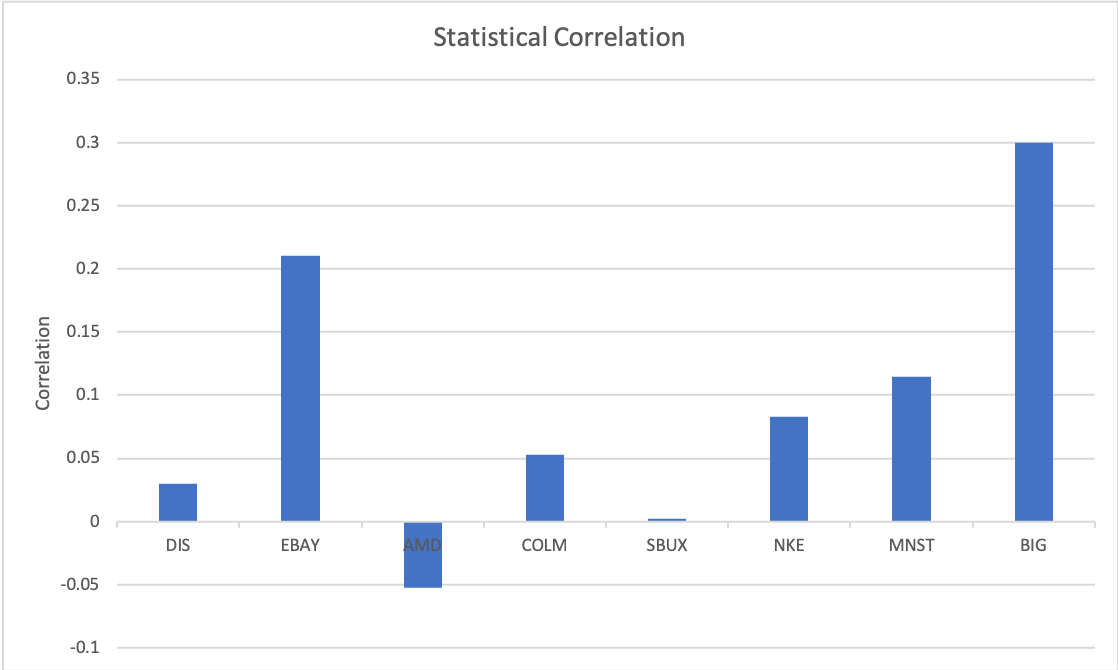
\includegraphics[width=120mm]{CorrelationResults.png}
\caption{Correlation Results \label{overflow}}
\label{Corrfigure}
\end{figure}

Because there is little correlation between closing price and average sentiment we should expect a na\"{i}ve strategy to perform poorly. We create a simple strategy that generates a buy signal when the average tweet sentiment is above .25 and generates a sell signal when it is below 0. We choose these values because of what we find in the data. Companies often have tweets that are positive, which is logical. Twitter is used as a means of promotion and sharing of news that is often positive so if the companies tweets for the day were on average negatively, we could expect the stock to perform poorly the next day. Figure~\ref{Naivefigure} shows the abysmal performance for this na\"{i}ve strategy. Only 25\% of the stocks end up beating the baseline, with the underperforming stocks performing terribly. EBAY characterizes the overall performance of this strategy well -- with the strategy returning 47.2\% while the baseline nets a 237.6\% profit. If sentiment was more correlated with closing price, we would expect this strategy to be more profitable. This lack of correlation motivates the need for a more sophisticated approach, such as using machine learning. 

\begin{figure}[h]
\centering
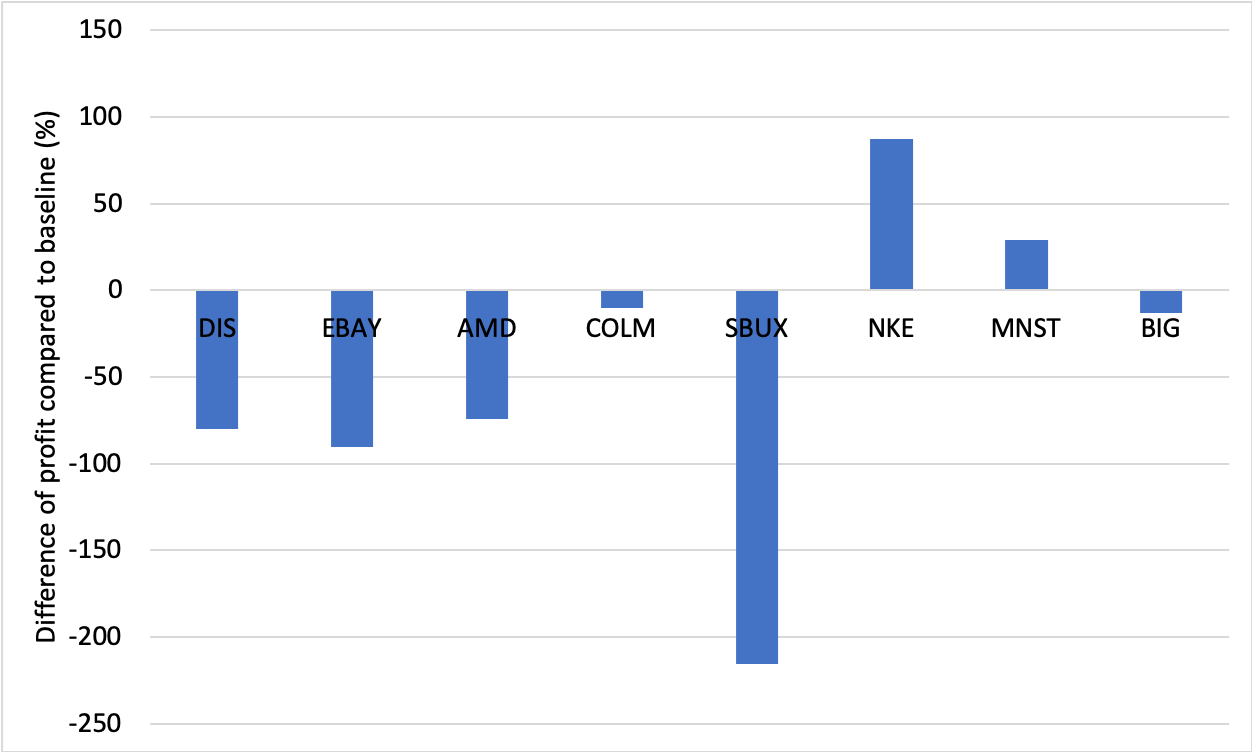
\includegraphics[width=120mm]{NaiveResults.png}
\caption{Naive Strategy Results \label{overflow}}
\label{Naivefigure}
\end{figure}


\section{Stock Trading and Machine Learning Algorithms}

Our implementation uses the both the Scikit-learn and TensorFlow Python libraries \cite{PedregosaFABIANPEDREGOSA2011} \cite{Abadi}. We use Natural Language Processing to conduct a sentiment analysis of tweets for our models. We then aggregate the twitter data across days of stock trading and then feed the combined stock and twitter data into a variety of different machine learning algorithms. \added[id=AT, remark = {this still needs to be worked on}] {WHY DO WE USE THIS VARIETY OF ML ALGOS?} We use this variety of machine learning algorithms to attempt to understand if one in particular works well with Twitter sentiment data or if the effectiveness of each algorithm varies from stock to stock. We discuss the different types of features inputted to these algorithms in section 6.4.

\subsection{Trees}

\subsubsection{Decision Tree Classifier}
Decision trees are models that predict the value of a target variable by learning simple decision rules inferred from the data features \cite{PedregosaFABIANPEDREGOSA2011}. It breaks down a dataset into smaller and smaller subsets, with the leaf nodes representing the classification prediction based on information gain. For features into the classifier, we use the default features specified in the Scikit-learn library. Specifically, we use a Gini impurity for criterion, we choose the best split, and use 2 as the minimum number of samples to split a node. Because we are using a classifier, our implementation predicts whether or not the following days closing price will be higher or lower, which is represented by a 1 or -1. Another benefit of decision trees is that they can be visualized easily. Figure~\ref{DecTreefigure} shows the decision tree fitted to DIS. However, due to the complexity of our model it is difficult to interpret the visualization. 

\begin{figure}[h]
\centering
\includegraphics[width=90mm]{decision_tree_DIS.pdf}
\caption{Decision Tree Visualization of DIS \label{overflow}}
\label{DecTreefigure}
\end{figure}

\subsubsection{RandomForest Regressor}
This module builds off of the above's section decision tree implementation. It instead uses a randomized decision tree making a diverse set of classifiers by introducing randomness in the classifier construction \cite{PedregosaFABIANPEDREGOSA2011}. This prediction of the ensemble is then given as an averaged prediction of the individual classifiers. Each tree in the ensemble when it is constructed is built from a random sample drawn from the training set. More randomness is added during construction by choosing the best split of nodes from a random subset of the features. This generally induces more bias from the randomness, but due to averaging often decreases variance and hence yields a better overall model \cite{PedregosaFABIANPEDREGOSA2011}. Just like the features used in the decision tree, we use the default values in the Scikit-learn library. We use 10 trees in the forest and measure quality of a split using mean squared error. Unlike a classifier, a regressor is able to predict and model float values, giving us a different insight, as our implementation predicts the magnitude of change in closing price rather than just the direction of price movement. 

\subsection{Other Classifiers}

\subsubsection{$K$-nearest Neighbors Classifier}
This algorithm is one of the simplest machine learning algorithms that exists. After choosing a $k$, or amount of nearest neighbors, it calculates the distance between the query sample and all of the training samples via Euclidian distance \cite{PedregosaFABIANPEDREGOSA2011}. The algorithm then sorts the ordered collection of distances and chooses the mode of the $k$ selected labels for classification. In a regression, it would choose the mean of the $k$ selected labels. For our  algorithm, we choose $k=5$. We do this because of the variety of different features that some of our models take will generate different groups of neighbors. Because we are doing classification, our algorithm predicts binary price change, as in the other classification algorithms discussed above. 

\subsubsection{MLP Classifier}
An MLP is a neural network of percpetrons that perform binary classification. They have an input layer, a certain number of hidden layers, and an output layer which makes a decision about the given input and are generally used in a supervised learning context. The network \textit{learns} by using a back-propagation algorithm consisting of two steps \cite{Honkela2001}. In the forward pass, predicted outputs from a given input are evaluated mathematically. In the backwards pass, partial derivatives of the cost function are propagated back through the network. Figure~\ref{MLPgraph} shows how a signal flows through a simple MLP with one hidden layer. 

\begin{figure}[h]
\centering
\includegraphics[width=90mm]{MLP_graph.png}
\caption{Signal-flow graph of an MLP \label{overflow}}
\label{MLPgraph}
\end{figure}

We choose a classifier with 3 hidden layers, each with 100 neurons, and use a stochastic gradient descent for the solver. While MLP classifiers can handle a variety of different layers and solvers, this combination proved to be most effective during testing of the algorithm for our combined Twitter and stock data. The MLP classifier predicts a 1 or -1, signaling a price rise or alternatively a price drop the following day. WHY DO WE DO THIS? not entirely sure


\subsection{Deep Learning}
We implement a Long Short Term Memory model (LSTM) using the TensorFlow Python library \cite{Abadi}. This is an example of a recurrent neural network (RNN). Unlike traditional neural networks, RNN's use previous data to help classify or predict the current value \cite{Colah2015}. RNN's have persistence and are networks with loops in them.  LSTM networks are a special type of RNN that is capable of learning long-term dependencies unliked traditional neural networks which struggle with this problem. They are trained via back-propogation over time and instead of neurons have memory blocks that are connected through layers. Each block contains 3 different types of gates which are triggered by sigmoid activation units: forget, input, and output gates. The first decides wether or not to throw away information from the block. The second decides which values from the input should be allocated to update the memory state. The third decides what to output based on input and memory state. Because the structure of an RNN allows the model to use past events to aid future states unlike a typical neural network, this has an ideal application for long term time-series based data, which makes an LSTM model ideal for our use case \cite{Colah2015}.

\added[id=AT, remark = {should i insert a graph?}] {should i give an explanation behind math/ graph??? - to be honest not entirely sure I understand it}

The model for our implementation has a look back of 60 days to give the model enough input to predict the following closing price. At its core, our LSTM model processes 60 days prior of inputs including closing price, tweet sentiment, and a variety of Twitter data, and then predicts the following days closing price. Unlike the above methods which predict signaled change, this model predicts the stock price. Furthermore, we add a second layer into our model. This stacked LSTM makes the output of the first layer become the input to the second layer, giving our model more depth and accuracy. To verify that our model is accurately predicting the following days stock prices well, we check the efficacy of the predictions by looking at mean squared error regression loss. This is done in Scikit-learn metrics function call to \texttt{mean\_squared\_error()}. 


\section{Models with Different Features applying Machine Learning Algorithms}

Each model, besides Deep Learning, run on the 4 different machine learning techniques described in the preliminaries: Random Forest Regressor, MLP classifier, decision tree classifier, and $k$-nearest neighbors classifier. We use a variety of different models to try to better understand the efficacy of particular machine learning techniques, or if a particular model is more effective than the others. For each model, all of the data is scaled using Sckit-learn's \texttt{minmaxscaler()} preprocessing tool to remove skew from the data. Most companies tweets aren't overwhelmingly negative and are far more positive. To test the effectiveness of the models, we trade with starting capital of \$1000. Using the predicted changes in price, we buy as many shares as possible when the price is predicted to close higher the next day. The strategy sells all shares when the price is predicted to close lower the next day. The baseline is obtained by buying \$1000 worth of shares at the beginning of the trading period and selling on the last day. 

\subsection{Simplistic Features}

The most simplistic model employed in our research only uses two inputs: closing price and average tweet sentiment.

\subsection{Complex Features}

Building on the simplistic features, we add other twitter features to the input. We use amount of tweets, favorites, and retweets to provide a more detailed input to the model, which should translate to more accurate results. 

\subsection{Stacked Features}

Using complex features, we use stacking to find more consistent performance with the particular machine learning algorithms. Stacking works by aggregating the buy or sell signal from each machine learning technique on each day of stock trading. We employ two different strategies -- one that behaves more conservatively and another that behaves generates buy signals far more leniently. The former sells all positions if any machine learning model generates a sell signal and only buys when all 4 models generate a buy signal. The latter gives a buy signal if more than half of the models generate a buy signal and sells if under half give buy signals.

\subsection{Deep Learning}

Our Deep Learning model uses complex features. As described above, we employ an LSTM neural network to predict stock price for the following day. To generate buy sell signals, we compare the predicted price to the current close. A positive difference signals a buy while a negative difference signals a sell just like the above models. 

\end{document}
